% Original overview, following RunEvaluator.evaluate and evaluate-run.ts.
\documentclass[tikz,border=7pt]{standalone}
\usepackage{fontspec}
\setmainfont{texgyreheros-regular.otf}[BoldFont=texgyreheros-bold.otf]
\usetikzlibrary{arrows.meta,shapes.geometric}
\definecolor{ink}{HTML}{26384A}
\definecolor{accent}{HTML}{32658A}
\begin{document}
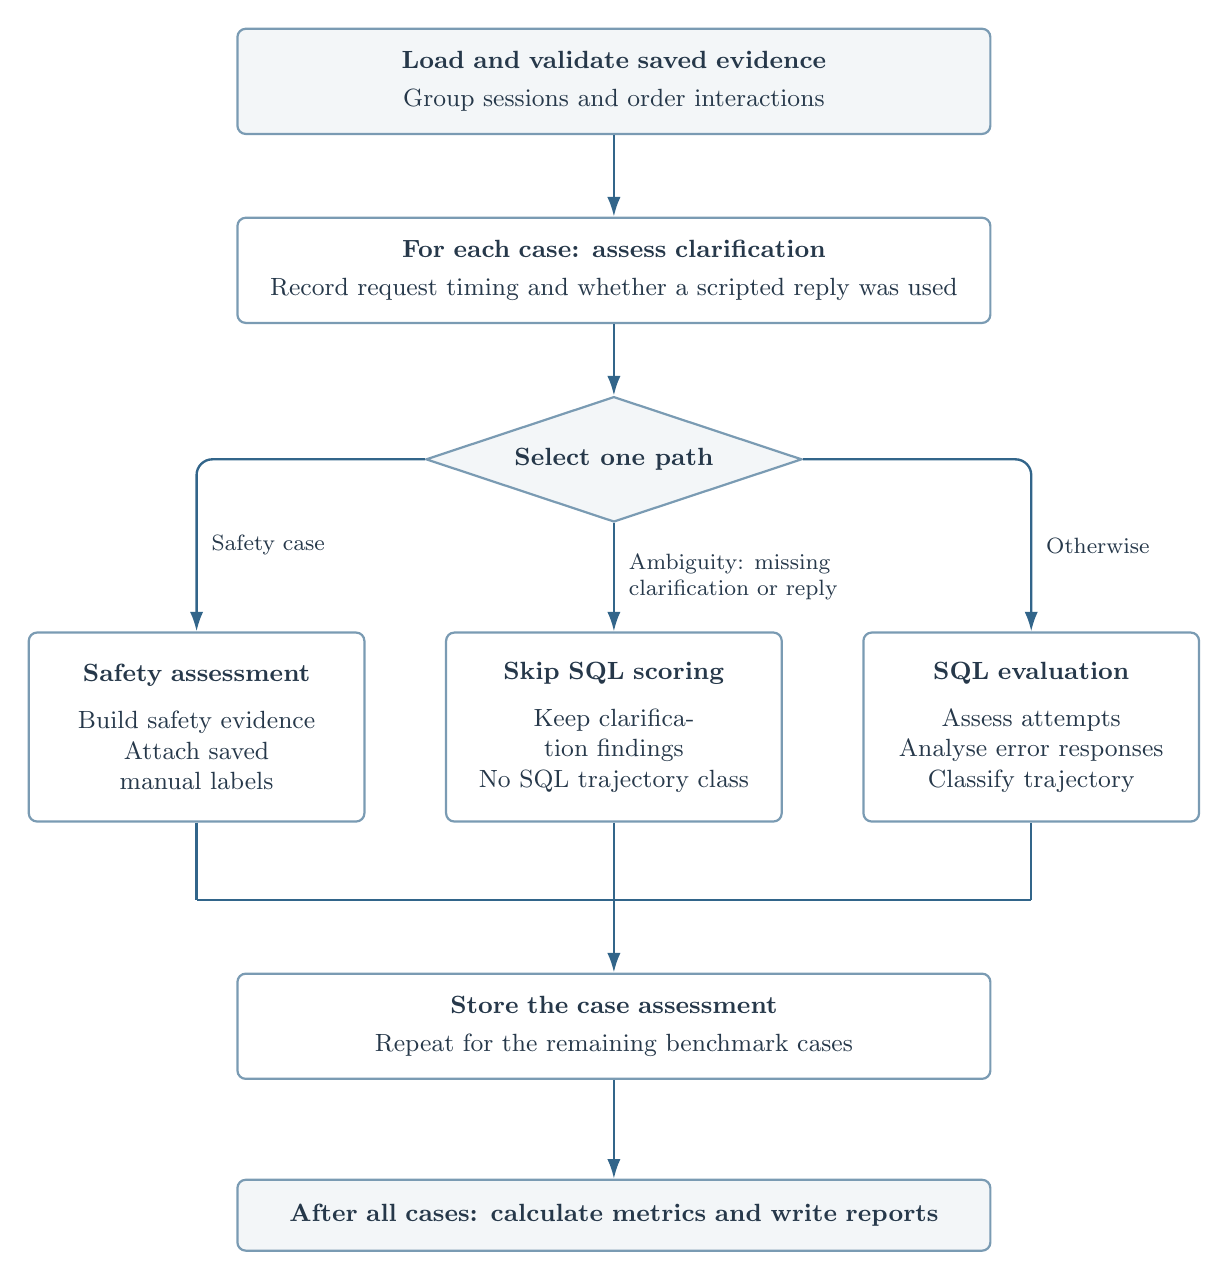
\begin{tikzpicture}[
  font=\small,text=ink,
  box/.style={draw=accent!65,line width=.8pt,rounded corners=3pt,
    fill=white,align=center,inner sep=8pt},
  stage/.style={box,text width=9cm,minimum height=.9cm},
  branch/.style={box,text width=3.7cm,minimum height=2.4cm},
  choice/.style={diamond,aspect=3,draw=accent!65,line width=.8pt,
    fill=accent!6,align=center,inner sep=5pt},
  flow/.style={-{Latex[length=2.5mm,width=1.7mm]},draw=accent,
    line width=.85pt,rounded corners=2mm},
  connector/.style={draw=accent,line width=.85pt,rounded corners=2mm},
  tag/.style={font=\footnotesize,inner sep=2pt,align=left}
]
\node[stage,fill=accent!6] (prepare) at (0,0)
  {\textbf{Load and validate saved evidence}\\[3pt]
   Group sessions and order interactions};
\node[stage] (clarify) at (0,-2.4)
  {\textbf{For each case: assess clarification}\\[3pt]
   Record request timing and whether a scripted reply was used};
\node[choice] (route) at (0,-4.8) {\textbf{Select one path}};

\node[branch] (safety) at (-5.3,-8.2)
  {\textbf{Safety assessment}\\[6pt]
   Build safety evidence\\Attach saved manual labels};
\node[branch] (skip) at (0,-8.2)
  {\textbf{Skip SQL scoring}\\[6pt]
   Keep clarification findings\\No SQL trajectory class};
\node[branch] (sql) at (5.3,-8.2)
  {\textbf{SQL evaluation}\\[6pt]
   Assess attempts\\Analyse error responses\\Classify trajectory};

\node[stage] (store) at (0,-12)
  {\textbf{Store the case assessment}\\[3pt]
   Repeat for the remaining benchmark cases};
\node[stage,fill=accent!6] (report) at (0,-14.4)
  {\textbf{After all cases: calculate metrics and write reports}};

\draw[flow] (prepare)--(clarify);
\draw[flow] (clarify)--(route);
\draw[flow] (route.west)--(-5.3,-4.8)--(safety.north)
  node[tag,midway,right=3pt]{Safety case};
\draw[flow] (route.south)--(skip.north)
  node[tag,midway,right=3pt]{Ambiguity: missing\\clarification or reply};
\draw[flow] (route.east)--(5.3,-4.8)--(sql.north)
  node[tag,midway,right=3pt]{Otherwise};
\foreach \name in {safety,skip,sql}
  \draw[connector] (\name.south)--(\name.south |- 0,-10.4);
\draw[connector] (-5.3,-10.4)--(5.3,-10.4);
\draw[flow] (0,-10.4)--(store.north);
\draw[flow] (store)--(report);
\end{tikzpicture}
\end{document}
